\section{Results}


\subsection{Smoothing Experiment}

In Section \S\ref{sec:modelingFluenceBlocking} we describe a smooth model of how the leaves block radiation.
Here we describe do a simple experiment to look at how adjusting that smoothing parameter affects the optimization.

We uses a single target fluence profile, as shown in Figure \ref{fig:fluenceMapSmoothingExample},
and assumes that the dose-rate is a constant function of time.
We performed a simple grid search, computing the optimal leaf trajectories for each dose-rate value.
We then ran this grid-search twice, once with heavy smoothing and once with light smoothing.

The smoothing parameter can be expressed in terms of a characteristic blurring width.
Here we used a width of 0.5 cm for the heavy smoothing and 0.05 cm for the light smoothing.
The characteristic width was computed such that the smoothing function achieved 95\% of its
change in value over the smoothing window.

We also used seven of leaf trajectory segments, although similar results are obtained for trajectories with more segments.
\todo{add a figure for that? Or maybe another sub-section?}
This number was computed with a pilot study.
Fewer trajectory segments lead to faster solve times, but the fitting error increases significantly.
Using more trajectory segments takes longer, but at a trivial reduction in fitting error.


\begin{figure}
  \centering
  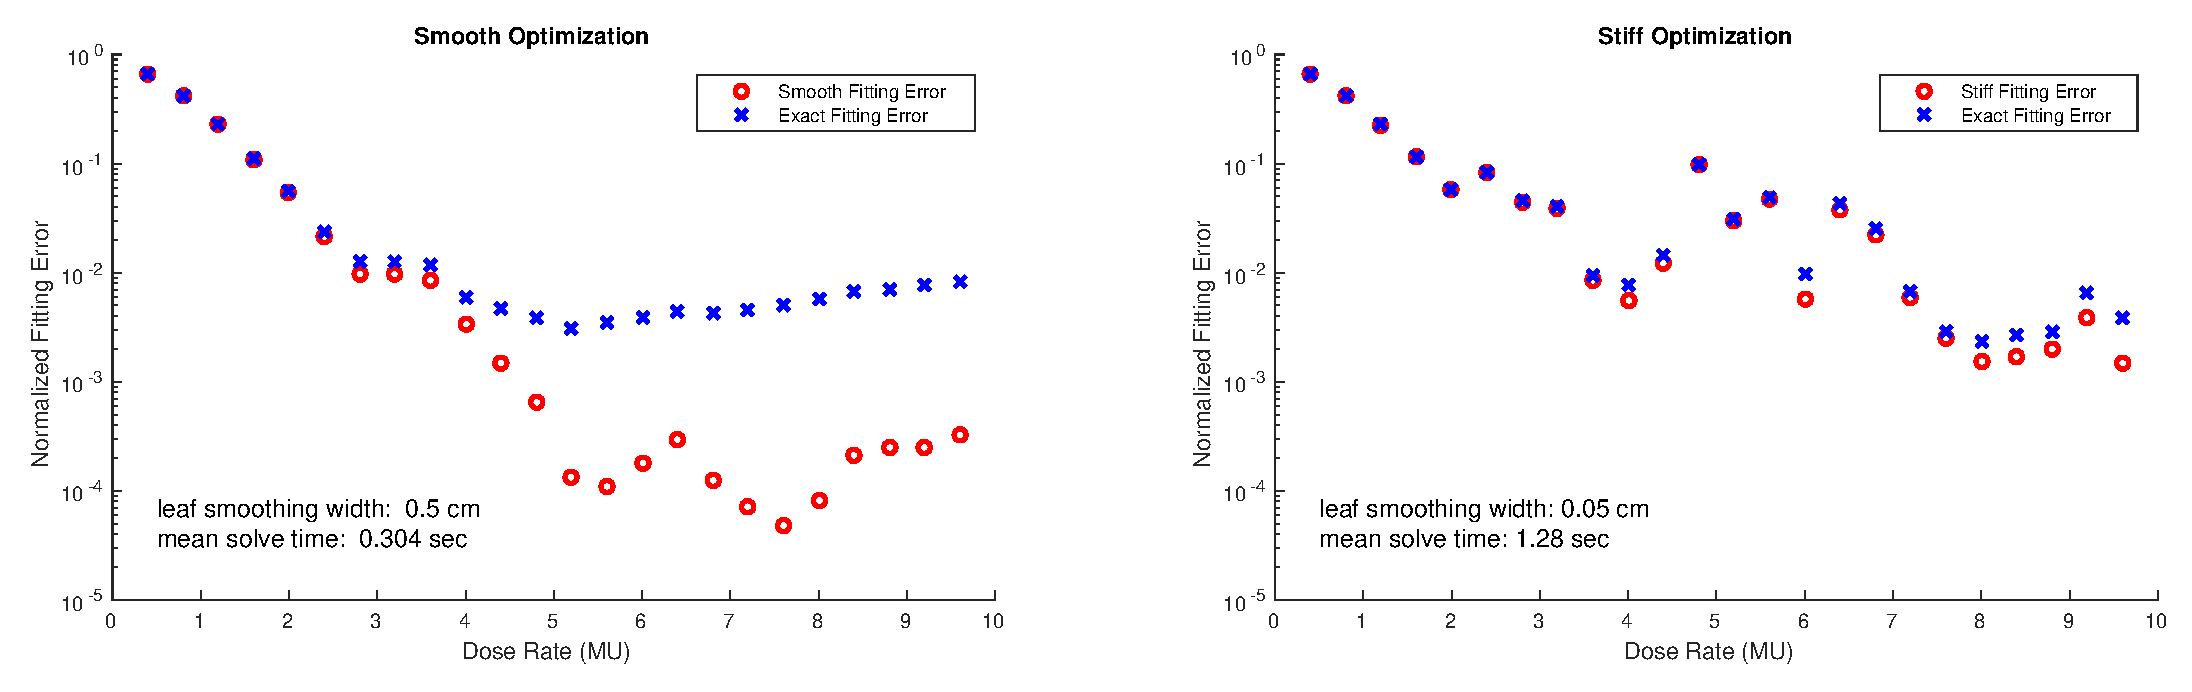
\includegraphics[width=\textwidth]{fig/smoothVsStiffOptimization.pdf}
  \caption{Smooth vs. stiff beaf-blocking model in optimization.
      In the optimization we smooth out the blocking caused by the edges of the leaves in the VMAT.
      A larger value of smoothing helps the optimization converge quickly and reliably, but with a
      loss of accuracy. Both plots show the leaf optimization for a sweep of constant dose rate
      trajectories. The left plot (\textit{smooth optimization}) uses a larger smoothing width of 0.5 cm,
      while the right plot (\textit{stiff optimization}) uses a smaller value of 0.05 cm.
      The stiff optimization takes about four times longer to run, and is a close match for the
      exact (non-smooth) model. The objective value does not vary smoothly as the dose rate
      increases, suggesting that the optimization is struggling with local minima.
      The smooth optimization runs faster and produces more consistent results as the dose rate changes.
      The fitting value predicted by smooth model is better than the exact model, but it is still
      a good fit, with the best solution being shown in \ref{fig:fluenceMapSmoothingExample}.
  }
  \label{fig:smoothVsStiffOptimization}
\end{figure}




\begin{figure}
  \centering
  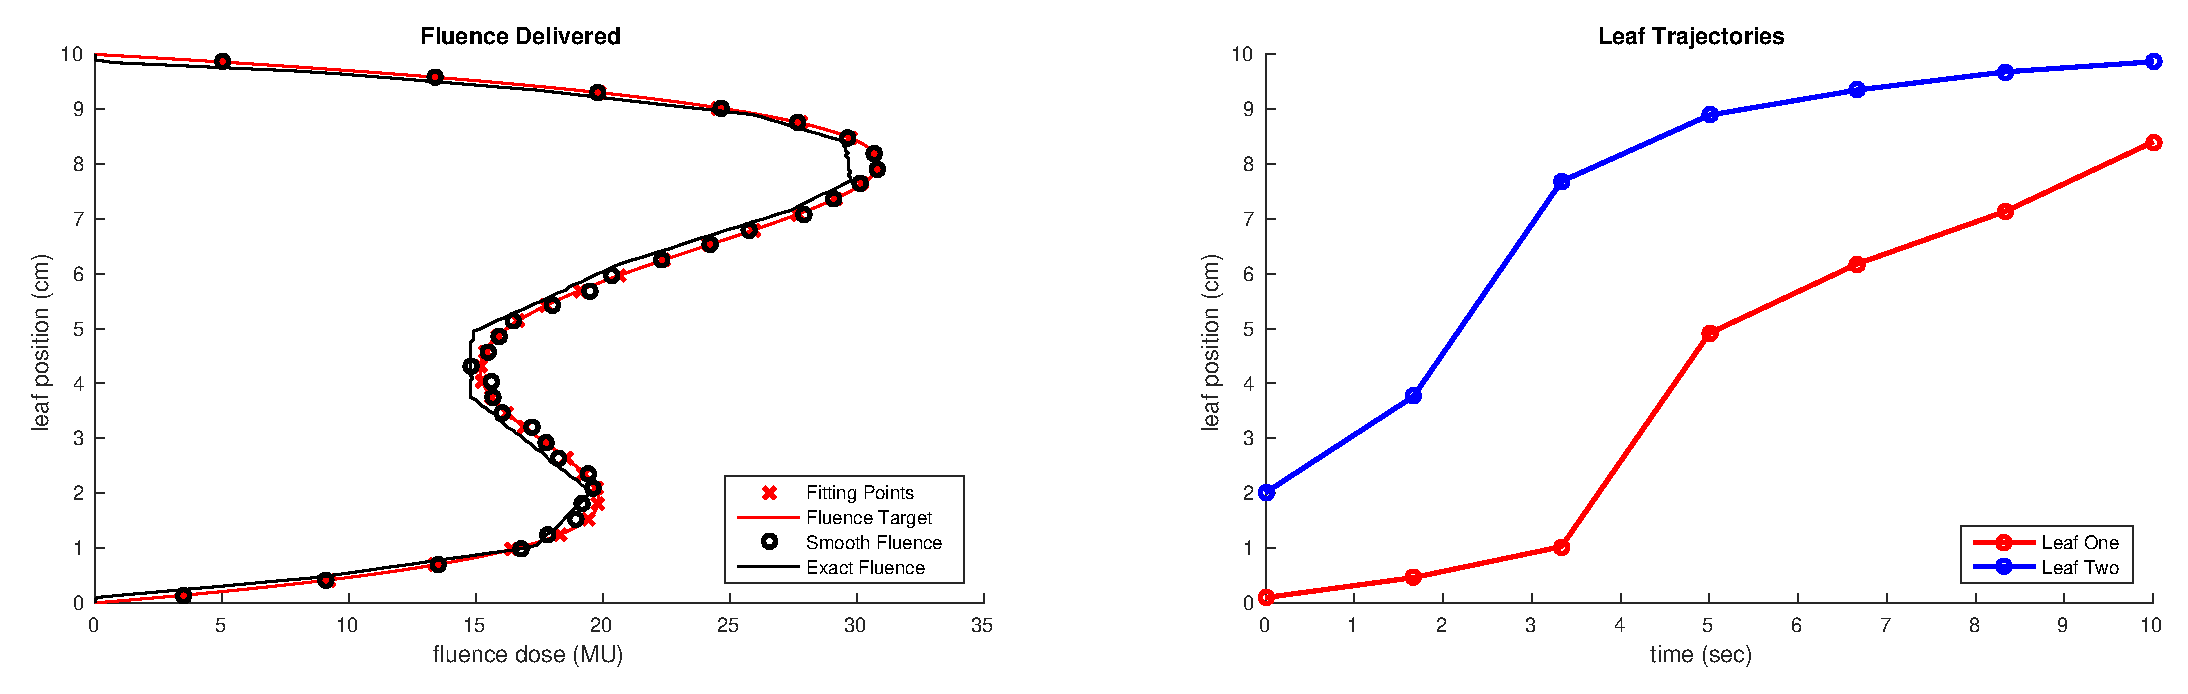
\includegraphics[width=\textwidth]{fig/fluenceMapSmoothingExample.pdf}
  \caption{Fluence fitting with a constant fluence dose rate of 5.2 MU,
      optimizing using the smooth model for leaf blocking, with a smoothing width of 0.5 cm.
      The optimization was able to achieve a very good fit with the smooth model, but the
      exact (no smoothing) value for the fluence delivered is also quite close.}
  \label{fig:fluenceMapSmoothingExample}
\end{figure}


\subsection{Iterative Smoothing reduction}


\begin{figure}
  \centering
  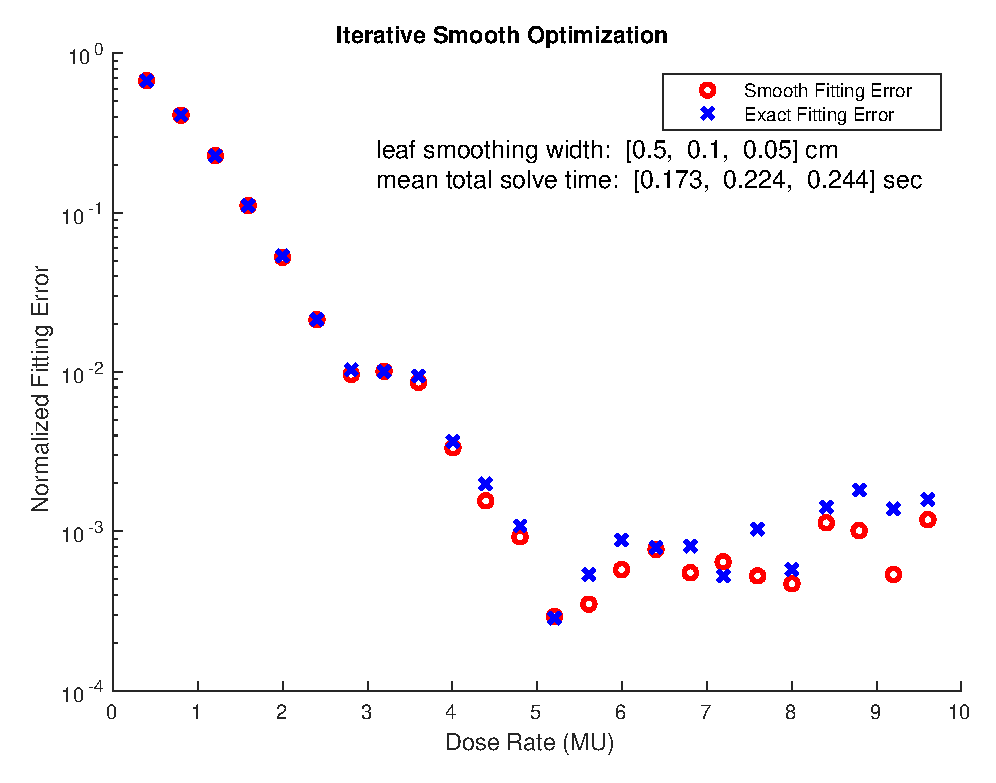
\includegraphics[width=3in]{fig/iterSmoothSweep.pdf}
  \caption{This plot shows the objective function value for the optimal leaf trajectories,
           given a constant fluence dose rate. Each optimization here is actually a set of three
           optimizations, each using a successively smaller smoothing distance. In all cases
           the first optimization used a smoothing distance of 0.5cm, the second used 0.1cm,
           and the final optimizaiton used 0.05cm. This technique results in faster solve times
           than a single optimization with the smallest smoothing parameter, while also avoiding
           local minima.}
  \label{fig:iterSmoothSweep}
\end{figure}




\begin{figure}
  \centering
  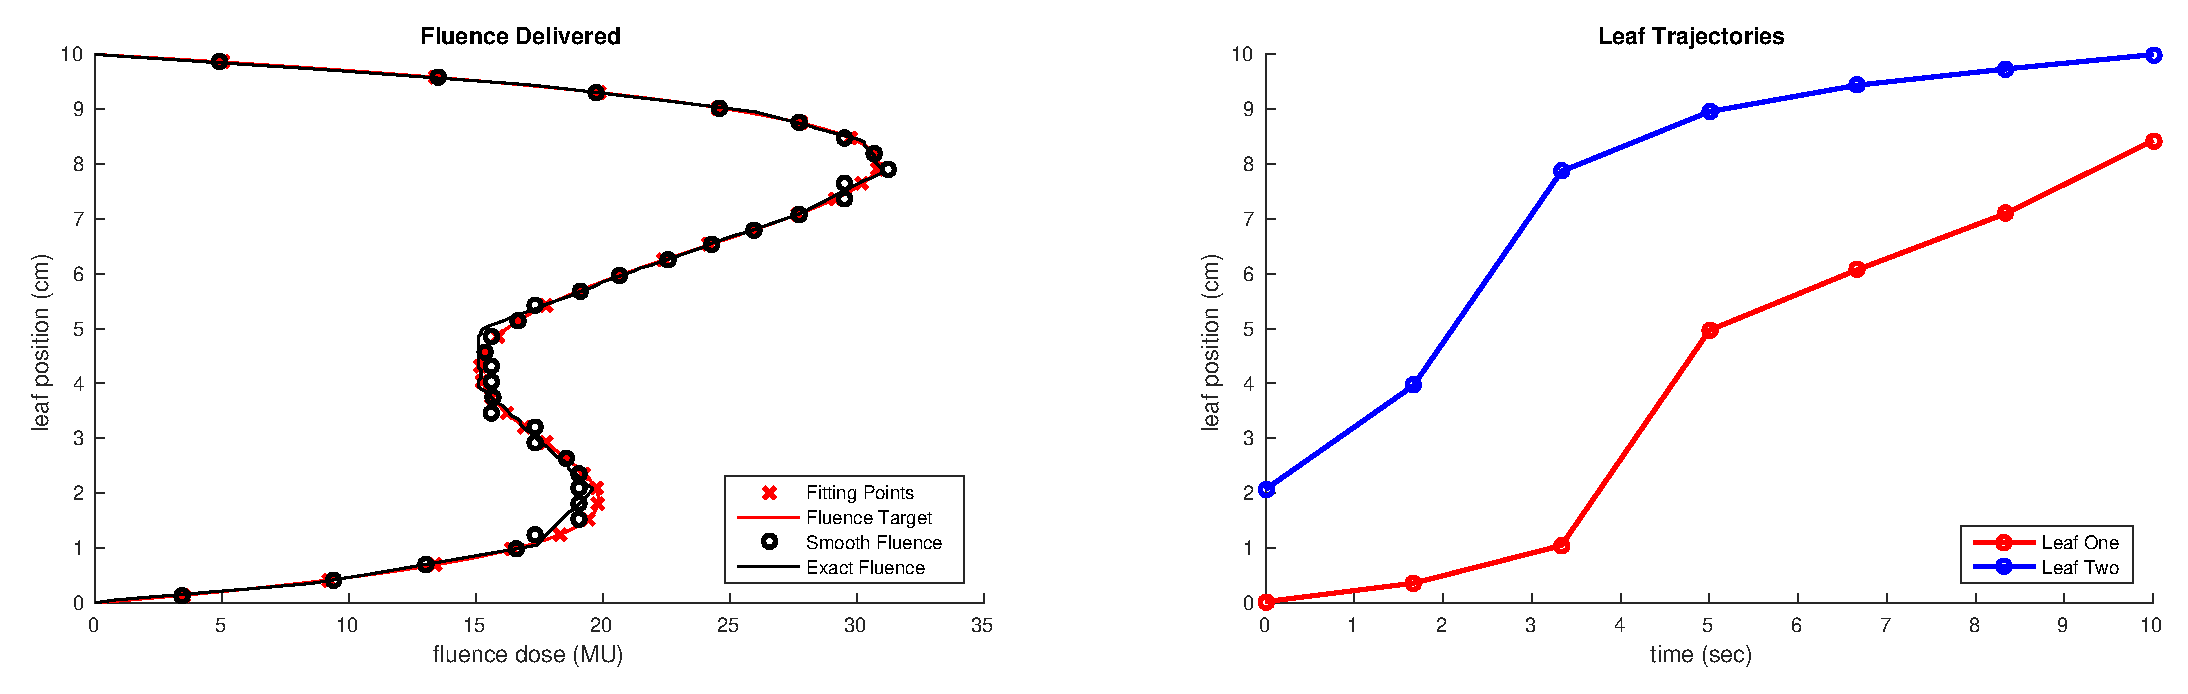
\includegraphics[width=\textwidth]{fig/fluenceMapIterativeBest.pdf}
  \caption{This plot shows the optimal leaf trajectories and delivered fluence map using the
           best solution (dose rate = 5.2 MU) found by the iterative optimization procedure.}
  \label{fig:fluenceMapIterativeBest}
\end{figure}



\subsection{Misc. Notes:}

It seems that the velocity smoothing has little effect on the optimization: no significant
change observed in computation time, convergence, or trajectories.

The number of fitting points is important -- if there are too few the the trajectories tend to
become less smooth and more local minima pop up. I believe that this is caused by overfitting.

The solve time varies linearly with number of trajectory segments, at least on the range of 7 to 13 segments.
The solution quality does not appear to change that much, although a few extra bumps do appear in the trajectories.
If there are too few points, then the it is sometimes not possible to capture some features in the target profile.
